\section{Evaluation}
\label{tach:sec:eval}

We have evaluated \tachyon with respect to three main
questions. First, can \tachyon detect deviations where the patched
program is semantically different than the unpatched, and how hard is
it to write rules to ignore deviations that do not matter? Second,
what is the performance factors for \tachyon, including best and worst
case settings? Third, what is the performance on real programs?  In
this section, we describe our results.

\subsection{Detecting Deviations}

To test the effectiveness of \tachyon, we used it on real patches
to detect known deviations.  The patches we tested are shown in
Figure~\ref{tach:fig:bug}. In this experiment, we tested the program on
normal inputs, and verified that \tachyon did not report a
deviation. We then tested on inputs that triggered known deviations,
e.g., exploits in the original program or bugs in the patch.

\begin{figure}
	\begin{center}
	\begin{footnotesize}
\begin{tabular}{|c|c|c|}
\hline
Program & Issue ID & Description\\
\hline \hline
cURL & CVE-2011-2192 & Improper key delegation\\
\hline
mplayer & EDB-ID 11792 & Table index out of bounds \\
\hline
php5 & CVE-2012-0832 & Bad Argument handling \\
\hline
php5 & CVE-2011-1938 & Buffer Overflow\\
\hline
ncompress & CVE-2001-1413 & Buffer overflow \\
\hline
htget & CVE-2004-0852 & Buffer overflow \\
\hline
gs & CVE-2010-1869 & Buffer Overflow\\
\hline
glftpd & EDB-ID-476 & Buffer Overflow\\
\hline
socat & CVE-2004-1484 & Format String\\
\hline
corehttp & CVE-2009-3586 & Off-by-one Buffer\\
\hline


\end{tabular}
\end{footnotesize}
\caption{Successfully Detected Deviations for Security Patches}
\label{tach:fig:bug}
	\end{center}
\end{figure}

% In these cases, the experiment performed was to first execute on several
% valid inputs the pre and post patch binary
% in order to check that no deviation was detected. Then, an input known to
% generate the erroneous behavior was fed into the patched system, and \tachyon
%  detected a deviation and terminated.

For cURL, the patched vulnerability was an information disclosure
bug. In the unpatched version, Kerberos credentials were (accidentally)
forwarded instead of just a proof the user was authorized.  We
verified that the unpatched program would send credentials, and the
patched program did not.  In order to test the patch and allow normal
operation of safe inputs, we had to write two rules for cURL that
totaled 11 lines.  The rules were necessary
because cURL added a non-security feature that affected file
descriptors in their patch.

% In cURL's case, the deviation appeared as a write with a different
% payload, which would trigger when attempting to talk to a Kerberos
% enabled server. The different payload was in fact a fully delegated
% credential rather than just what was required to make the connection
% and authenticate. In the other cases, the deviation appeared as a
% non-synchronized program termination, except when a proper exploit was
% available, in which case it appeared as one program making a
% legitimate system call, as the other tried to call
% \texttt{system("/bin/sh")}.


CVE-2011-4885 addresses a problem in PHP where hash collisions are
easy to find, which can be used to launch a remote denial of service
attack. \tachyon required no rewrite rules
to run the patch on safe inputs.  The patch, however, broke the
argument handling for arrays after loading many
arguments. CVE-2012-083 addressed this problem.  For CVE-2012-083, we
again required no rewrite rules for safe inputs.

CVE-2011-4885 and CVE-2012-0832 demonstrate a patch that is broken,
and provide motivation for \tachyon. Since CVE-2011-4885 fixed a
purported vulnerability, it should be applied immediately. However,
after applying CVE-2011-4885, a \emph{new} vulnerability is
introduced. \tachyon detects those new exploits as deviations
immediately. In particular, we checked exploits (addressed in
CVE-2012-0832) that were unknown in 2011, and verified that they
caused detected deviations. Thus, if an administrator had been running
\tachyon, and immediately applied the patch, they would detect
exploits immediately against the vulnerability introduced.


The EDB-ID 11792, CVE-2001-1412, and CVE-2004-0852 all patch typical
security bugs by adding inline checks. These checks did not change the
system call pattern or arguments, thus no rules were needed for patch
testing.

For CVE-2010-1869, \texttt{gs}'s memory problems required a rewrite rule
to admit additional or skipped calls to $\texttt{brk}$.
8 lines were required for these rewrite rules. Three lines were required
for EDB-ID-476 to allow for rewriting of the format of a usage
message. Four were required to deal with the new \texttt{lstat}s in the patch for CVE-2009-3586.

\subsection{False Positive Testing}
To show that \tachyon is fairly precise, we tested it on the most recent 207 patches to coreutils. (The number 207 was chosen because that was how far backwards we could go easily with an automated building system.) From this, we found that in 18 cases out of 1656 executions, a deviation was reported, or \tachyon crashed. Looking at the output, 16 of these were \tachyon bugs, but are not systematic, so that re-running the test produced correct results. 2 of these were actual deviations. In the first, a call to \texttt{fadvise()} was introduced into \texttt{cp}. An equivalence can be reached with a one-line rewrite rule. In the second, a buffer size was changed. The read/write splitting/coalescing rules described earlier in this chapter allow an equivalence to be reached. Overall, this indicates that while \tachyon is not perfectly bug free, it never reported a deviation when one had not happened, and deviations that should be acceptable could be easily expressed in the rule system.

We also ran \tachyon on patches for two common utilities with no known
vulnerabilities:
\texttt{/bin/ls} and \texttt{/bin/cat}, and used them interactively.
In the one month testing period, \tachyon was able to use tandem
execution on these utilities for normal day-to-day use with no
perceived slowdown. Further, \tachyon
reported no deviations (i.e., had no false positives).

\subsection{Micro-benchmarks}


\tachyon has three main sources of overhead: our approach to syscall
interposition, transferring bytes from the source to the sync
application, and running both $\unpatched$ and $\patched$
in tandem. Overall we measured a linear overhead for both data transfer and
system calls, and 0\% of CPU time, as detailed below.


\paragraph{Syscall interposition overhead.} \tachyon is a user-space
system call interposition scheme, which imposes additional context
switches but provides for a clean separation of interposition, kernel,
and user-space application.  Our user-space interposition has 4 context
switches per call issued by the live application $\patched$. For each
syscall in $\patched$, \tachyon context switches from $\patched$ to
the kernel, from the kernel to \tachyon, from \tachyon back to the
kernel, and finally back to $\patched$. Normal operation only has two
context switches: from user to kernel space, and back again.


In order to test the effect of these two extra switches, we wrote a simple
program that executed \texttt{getpid()} in a tight loop.
We were sure to call the system call directly, as the standard version of
\texttt{getpid()} in C actually caches its result.


\paragraph{Data copy overhead.} \tachyon needs to copy the output data
from $\patched$ to $\unpatched$.  A first naive implementation
actually incurred 6 copies.  \tachyon originally copied output data
from $\patched$ into \tachyon for syscall rewriting, and then copied
it to $\unpatched$.  Each copy between systems was actually two
copies: one from the user-space into kernel space, and one from
kernel-space into user-space. This lead to a huge slowdown in early
benchmarks (over 6x).  To reduce this, we added the ability to the
Linux kernel to map a remote process's memory via
\texttt{/proc/pid/mem} under most situations, making the normal case
of reading from the remote process only have one copy.


\begin{figure*}
\begin{minipage}[b]{0.49\linewidth}
\centering
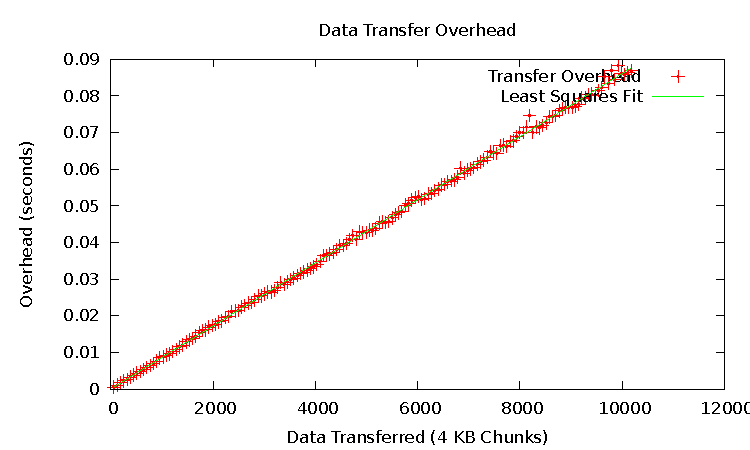
\includegraphics[scale=0.5, trim=40mm 0mm 20mm  0mm]{tachyon/dataData.pdf}
\caption{Data Transfer Overhead}
\label{tach:fig:dover}
\end{minipage}\begin{minipage}[b]{0.49\linewidth}
\centering
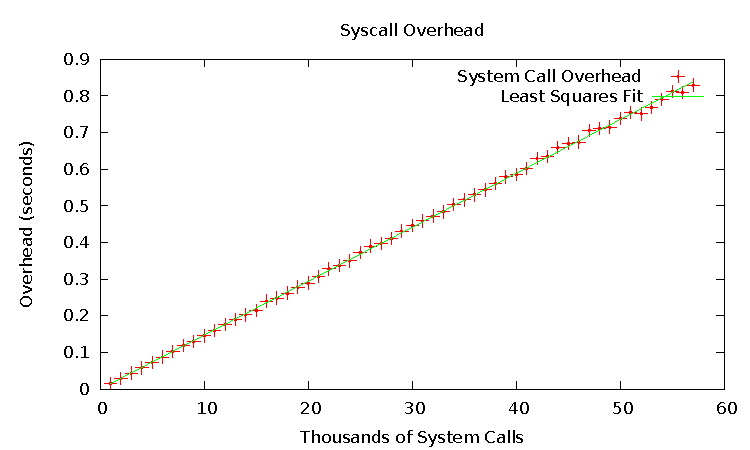
\includegraphics[scale=0.5]{tachyon/sysData.pdf}
\caption{Syscall Overhead}
\label{tach:fig:sover}
\end{minipage}
\end{figure*}

In Figure \ref{tach:fig:dover}, we see the overhead is in a linear relationship.
The overhead here is the total overhead
time for the system. While they make a difference for small data transfers, they are
rapidly dominated. This can be seen by the rapid transition to a tight grouping
around a linear relationship.


In Figure \ref{tach:fig:sover}, we again observe a nice linear relationship, showing no residual effects on performance from processing a system call. It shows that it takes less than a second of overhead to process 60,000 syscalls.

When varying the CPU load of the traced program, no noticeable difference in execution time was noticed, as we do not intercept regular computation, only system calls.

Given this, if it is known how many system calls are used, how much data is being
transferred, and how much time is being spent on the CPU, we can model how long
a given workload would take under our tracer.
\tachyon previously incurred a large number of copies and control transfers to move buffers around
in comparison with the register fetching it does for simple system calls, and
the remote memory fetch path is not optimized in the OS. However, a kernel patch
allowing for \texttt{mmap} to be used on the special file \texttt{/proc/pid/mem}
considerably ameliorate this, resulting in the new statistics above.

\paragraph{Tandem execution CPU time.}
The final source of overhead is in CPU operations.  Since \tachyon
sleeps when system calls are not being issued, it does not slow down
applications that are CPU-intensive. This is a significant advantage
over instruction-level interposition tools such as Pin~\cite{luk:2005} and
Valgrind~\cite{nethercote:2003:valgrind}, which typically suffer at least several
times overhead.

However, we are running both $\unpatched$ and $\patched$. We verified
that \tachyon can utilize independent cores to run both programs with
no additional overhead (other than the memory transfer and syscall
overhead measured above). Thus, we conclude that \tachyon can utilize
multi-core to test patches.

\paragraph{Efficiency on real programs.}

To test the efficiency of \tachyon interposition, we measured its
tandem execution against \texttt{strace} and \texttt{gdb}'s reverse
execution.  {\tt strace} is a tool built on top of \texttt{ptrace}
used to monitor system calls.  \texttt{gdb} allows programs to
back-step through operations.\footnote{We were unable to test against
  what is likely the most similar system, R2~\cite{guo:2008}, as it is
  both Windows only and requires build-time support (as well as not
  being public).} Note these tools have different goals than \tachyon;
we only use them to evaluate performance.

\texttt{gdb}'s replay mechanism derived from its reversible debugging
support. However, it proved wholly unsuitable for regions of more than
a few instructions. Due to a lack of SSE support, memcpy would be
improperly rewound and replayed. Additionally, even then the recording
overhead was more than 100x native execution, and built up a huge
memory data structure, making it impractical to benchmark.

\begin{figure}
\begin{small}
	\begin{center}
\begin{tabular}{|c|c|c|c|c|c|c|c|}
\hline
Program & Load & \tachyon  & \texttt{strace} \\
\hline \hline
\texttt{compress}  & 32M Random & 1.41  & 19.78 \\
\hline
\texttt{primegaps} & First 35 & 1.00 & 1.00 \\
\hline
\texttt{mencoder}  & h264 & 1.07 & 1.12\\
\hline
\end{tabular}
\end{center}
\end{small}
\caption{Tracing Performance (relative to native execution)}
\label{tach:fig:strace}
\end{figure}

The results compared to \texttt{strace} are shown in
Figure~\ref{tach:fig:strace}.  Overall, \tachyon was faster, sometimes by a
large margin, than a comparable syscall interposition scheme. 
This is partially because \tachyon can and does process some of its overhead while the traced program is doing work, but mostly due to the massively improved facility for retrieving remote memory via our patch to mmap /proc/pid/mem.

\paragraph{Web Server Tests.} We also tested the throughput of
\texttt{lighttpd} and \texttt{thttpd} when monitored under \tachyon.
In this test, we use ApacheBench (ab) configured to make 1000 requests
in two threads, downloading 4096 byte web page.  We ran the experiment
in two scenarios: on localhost and across the Internet.  

In the network experiment, the web servers ran at one university, and
requests were made from another university on the opposite US coast.
There was no detectable degradation for \texttt{thttpd}, and only
about a 30\% slowdown for \texttt{lighttpd}. Essentially, what this
shows is that while the system does not deal well with applications
whose progress is primarily based on the rate at which they can issue
system calls, when we move closer to a real deployment, applications
do not tend to have that as their primary limiting factor.

In the second experiment, we ran ab on localhost.  This is a
worst-case test because both web servers spin in a tight loop on a
syscall (\texttt{lighttpd} spins on \texttt{epoll}, and
\texttt{thttpd} on \texttt{poll}). 
This creates a pathological case for \tachyon, because the application
spends most of its time neither doing IO, nor doing computation, but
instead spends most of its time moving across the system call barrier.

\tachyon
took 8.9 times longer on $\texttt{lighttpd}$ (throughput decreased to
10\% of original values) and 14.2 times longer on $\texttt{thttpd}$
(throughput decreased to 7\% of original values).

To round things out, we also ran a test over a few hops on the local network.
As expected, intermediate results were measured to be between the two, with
1.17 times untraced completion to complete the test with $\texttt{thttpd}$, and 3.72
times untraced completion to complete the test with $\texttt{lighttpd}$.

With a more real network (or a more complicated webapp), we can see the
slowdown is lessened. With a real network, \texttt{epoll} will spend more
time waiting, diminishing the perceived effects.

% \texttt{mencoder} was run in a record only mode, as
% it aggressively uses all available cores, and so attempting to run two copies in
% tandem (which none of the other tracing utilities do) will necessarily produce
% massive overhead, and not truly measure the overhead of \tachyon.



%%% Local Variables: 
%%% mode: latex
%%% TeX-master: "paper"
%%% End: 
